\chapter{Marco investigativo}\label{cap2:Marco-Investigativo}

\section{Definición de conjunto de datos o dataset}

Una definición de aprendizaje automático es la siguiente : \medskip

“El machine learning traducido al español como aprendizaje automático es un subcampo de la 
Inteligencia Artificial que busca como construir programas de computadora que mejoran 
automáticamente adquiriendo experiencia” \cite{Arang} pág. 320 . \medskip

Usaremos indistintamente como sinónimo en lo futuro , “aprendizaje automático”   y  “machine learning”.

\begin{figure}[ht]
  \centering
  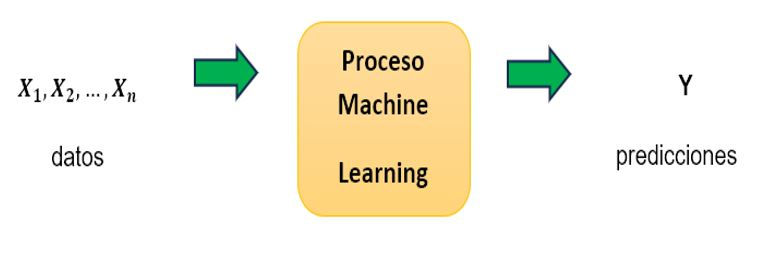
\includegraphics[width=10cm]{Imagenes/EsquemaML.JPG}
  \caption{Esquema Machine Learning}
  \label{fig:EsML}
\end{figure}

Un algoritmo de aprendizaje automático acepta como entrada un conjunto de datos también 
llamados dataset y después de un proceso realiza predicciones con estos datos \ref{fig:EsML} .\medskip



A la tabla completa de la Figura \ref{fig:Tblml}  la llamamos conjunto de datos (dataset), 
a las columnas en color amarillo le llamamos características y a la columna en color azul 
le llamamos variable objetivo y también se la conoce como etiqueta. \medskip

Como mencionamos anteriormente el aprendizaje supervisado cuenta con la columna de etiqueta y 
el aprendizaje no supervisado, no cuenta con esta columna.\medskip

Si la variable objetivo o característica son valores discretos , entonces le llamamos un 
problema de clasificación. Y si es un valor continuo le llamamos un problema de regresión.\medskip



De forma general los tipos de aprendizaje automático se pueden clasificar de la         
siguiente manera:\medskip

\begin{figure}[H]
    \centering
       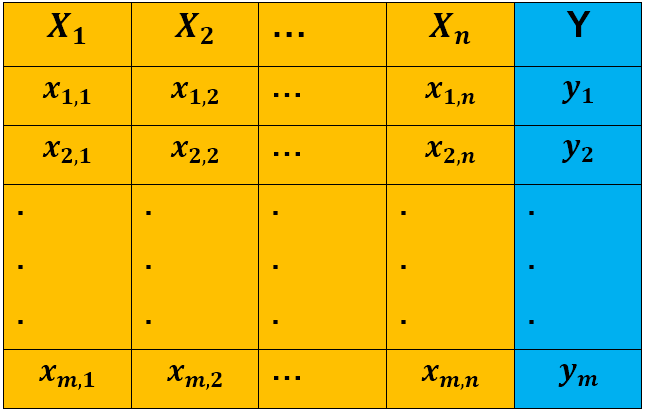
\includegraphics[width=12cm, height=7cm ]{Imagenes/TablaML.PNG}
      \caption{Conjunto de datos o dataset}
      \label{fig:Tblml}
  \end{figure} 


\subsection{Aprendizaje supervisado}
El modelo aprende con datos etiquetados, donde cada entrada tiene una respuesta conocida.\medskip

\subsection{Aprendizaje no supervisado}
El modelo trabaja con datos no etiquetados, descubriendo patrones y estructuras por sí mismo.\medskip


Estos tipos de aprendizaje ofrecen estrategias distintas para abordar desafíos en machine 
learning, cada uno con sus propias aplicaciones y utilidades específicas.\bigskip


\section{Clasificación}

La clasificación es un modelo supervisado en la cual el objetivo es predecir una 
etiqueta o clase para una entrada dada. En otras palabras, el modelo debe 
asignar una etiqueta categórica a las instancias basándose en características o 
atributos de los datos. \medskip

El modelo examina las características o atributos de los 
datos de entrada y crea una función o regla que relaciona esas características con la 
etiqueta de salida deseada. El objetivo final es que el modelo pueda generalizar esta 
relación aprendida para hacer predicciones precisas sobre nuevos datos no etiquetados. \medskip

En la Figura \ref{fig:Clasi} se muestra un ejemplo de un problema de clasificación de datos 
en dos o mas conjuntos que se relacionan con base en algunas características. La figura fue generada con 
ayuda del software Scikit-learn que puede graficar diferentes modelos de machine learning.


  \begin{figure}[H]
    \centering
       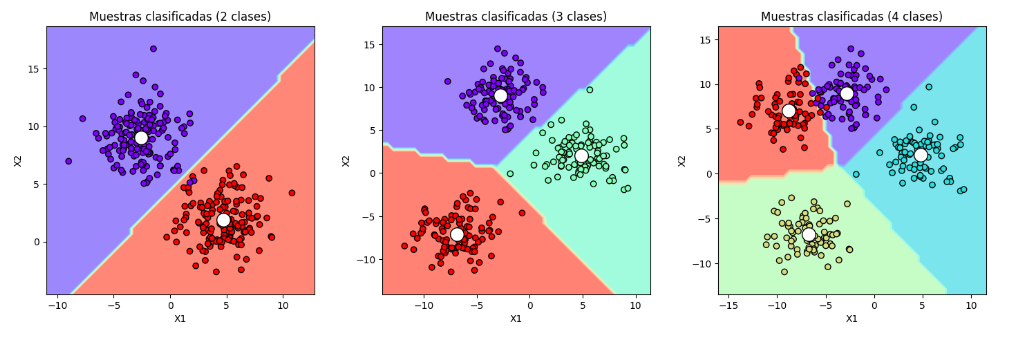
\includegraphics[width=12cm , height=5cm]{Imagenes/Clasificacion.PNG}
      \caption{Clasificación de un conjunto de datos}
      \label{fig:Clasi}
  \end{figure}
 

\section{Agrupamiento o Clustering}

El clustering o agrupamiento es un modelo no supervisado donde 
el objetivo es agrupar un conjunto de objetos en grupos, 
de manera que los objetos en el mismo grupo (o cluster) sean 
más similares entre sí que con los de otros grupos.\medskip

En la \ref{fig:Clast} se muestra un ejemplo de agrupamiento de datos 
usando el software Scikit-learn.


\begin{figure}[H]
    \centering
    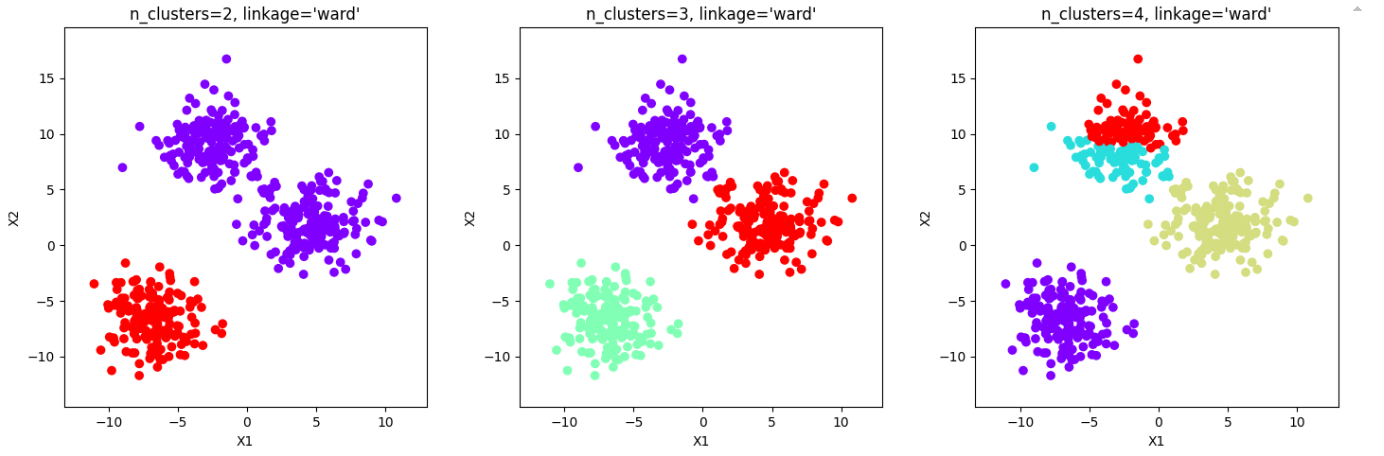
\includegraphics[width=12cm]{Imagenes/Clustering.PNG}
    \caption{Clustering o agrupamiento}
    \label{fig:Clast}
\end{figure}

\section{Regresión}
La regresión, es un modelo supervisado que busca entender la relación entre dos o más 
variables. En particular, se centra en proveer o regresar un valor numérico 
(la variable dependiente) en función de otras variables 
(llamadas variables independientes o predictores). \medskip

La regresión trata de encontrar la mejor línea o curva que represente la tendencia 
general de los datos. Esta línea o curva permite hacer predicciones sobre el valor de la 
variable dependiente cuando conoces los valores de las variables independientes. 
La figura \ref{fig:Reg1}  muestra varios tipos de regresión que modelan 
diferentes conjuntos de datos.\medskip



\begin{figure}[H]
    \centering
       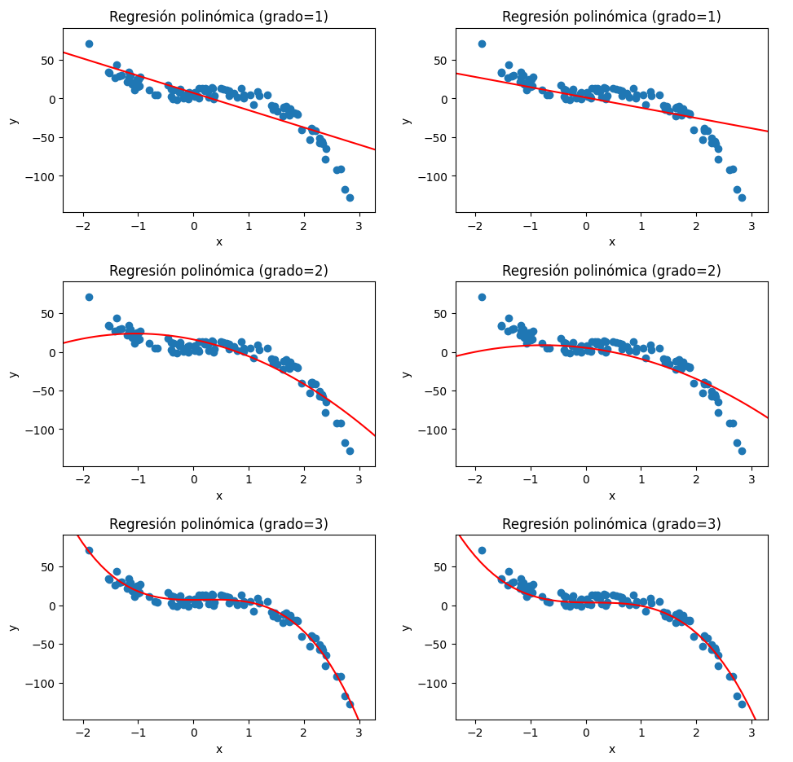
\includegraphics[width=10cm]{Imagenes/Regresion1.PNG}
      \caption{Regresión}
      \label{fig:Reg1}
\end{figure}



\section{Reducción de Dimensionalidad}

La reducción de dimensionalidad es una técnica fundamental en el análisis de datos que busca 
simplificar conjuntos de datos complejos manteniendo la mayor cantidad posible de información 
relevante. Una de las metodologías más populares para lograr esto es el 
Análisis de Componentes Principales (PCA, por sus siglas en inglés). \medskip

El Análisis de Componentes Principales (PCA) es una técnica estadística que se utiliza para 
reducir la cantidad de variables en un conjunto de datos mientras se conserva la mayor 
cantidad de variación en los datos originales. PCA transforma los datos originales en un 
nuevo sistema de coordenadas basado en componentes ortogonales, llamados componentes principales,
que son combinaciones lineales de las variables originales. \medskip

La reducción de  la dimensionalidad de los datos por lo tanto nos ayuda a 
simplificar el modelo matemático y, a su vez, disminuir los recursos computacionales, como 
el tiempo y el espacio de almacenamiento.\medskip



